\documentclass[11pt, oneside]{article} 
\usepackage{geometry}
\geometry{letterpaper} 
\usepackage{graphicx}
	
\usepackage{amssymb}
\usepackage{amsmath}
\usepackage{parskip}
\usepackage{color}
\usepackage{hyperref}

\graphicspath{{/Users/telliott/Dropbox/Github-Math/quickgeo/figures/}{/Users/telliott/Dropbox/Github-Math/figures/}}
% \begin{center} \includegraphics [scale=0.4] {gauss3.png} \end{center}

\title{Euler line}
\date{}

\begin{document}
\maketitle
\Large

%[my-super-duper-separator]

Draw a circle with center $O$, then draw a triangle ($\triangle ABC$) circumscribed by the circle.  The point $O$ is the circumcenter of the triangle, since the circle is its circumcircle.

Recall that to find $O$, given the triangle, we erect the perpendicular bisector from two sides and find the point where they meet.  It is easy to show that the perpendicular bisector from the third side meets the same point.

It is also easy to show that the converse is true.  The point $M$ below $O$ with $OM \perp BC$ is the perpendicular bisector of that side.

\begin{center} 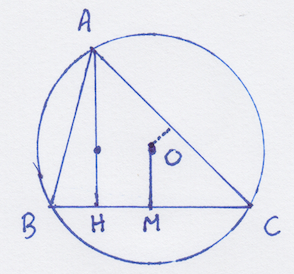
\includegraphics [scale=0.6] {EU1.png} \end{center}

The orthocenter $K$ is the point where the altitudes meet ($AH \perp BC$), see the next figure.  Only one altitude is shown.  

It is also one-third of the distance up from the base.  We showed this in the case of an equilateral triangle previously, and give a more general proof below.  That fact will become crucial in this proof.

Now draw the line from the upper vertex that bisects the base $M$.  Assume that we can draw the other medians of the triangle and find the point $G$ where they meet.  

Alternatively we can find the point $G$ numerically such that $GM$ is one-half of $AG$.  We revisit the proof for this below as well.

\begin{center} 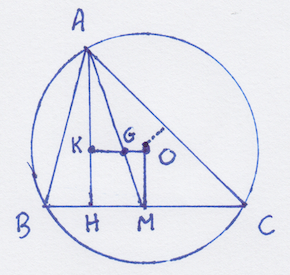
\includegraphics [scale=0.6] {EU2.png} \end{center}

So then we have three points $K$, $G$ and $O$ that we claim are co-linear.  What that means is that if we draw $KGO$ all three points lie on a straight line.  

\emph{Proof}.

First draw draw $KG \perp OM$. By similar triangles, since $AG$ is twice $GM$, $AK$ is twice $KH$.  But the orthocenter has the same ratio.  Hence $K$ is the orthocenter of the triangle.

So then extend $KG$ to meet $OM$.  The question is, why does $KG$ go through point $O$?

$\square$

For the medians and the point where they meet (called the centroid) recall Menelaus' theorem.  Applied to the centroid, we have
\[ \frac{x}{y} \cdot \frac{b_1}{b_2} \cdot \frac{c}{c_2} = 1 \]

\begin{center} 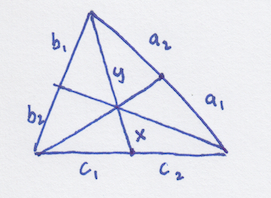
\includegraphics [scale=0.6] {K6.png} \end{center}

But $b_1 = b_2$ and $c$ is twice $c_2$ so
\[ \frac{x}{y} \cdot 2 = 1 \]

We conclude that $y = 2x$.

For the altitudes, we use an argument based on similar triangles.
\begin{center} 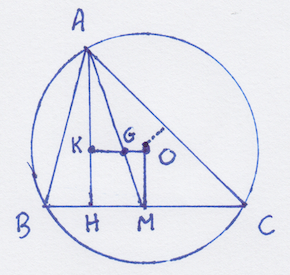
\includegraphics [scale=0.6] {EU2.png} \end{center}

$\triangle AKG \sin \triangle OGM$.  The ratio of sides is $2:1$ based on the centroid.  Therefore $AK/OM$ is also $2:1$.  

But $KH \parallel OM$, $OK \parallel BC$ and $OM \perp OK$, so $KH = OM$.  The ratio of $AK$ to $KH$ is also $2$.

$\square$







\end{document}
